\section{Declarative goals and domain properties\label{section:background-goals}}

A \emph{goal} is a prescriptive statement of intent, whose satisfaction requires the collaboration of agents forming the system. Unlike goals, \emph{domain properties} are descriptive statement about the environment -- such as physical laws, organizational rules, etc. Goals are structured in AND/OR refinement graphs showing how they contribute to each other~\cite{VanLamsweerde:2000}.

Section~\ref{subsection:background-goals-as-fltl-assertions} formalizes goals and domain properties in fluent linear temporal logic (FLTL). Their integration with state machines and scenarios is discussed in Section~\ref{subsection:background-goals-consistency}. Section~\ref{subsection:background-property-and-tester-automata} then presents how all system traces satisfying (resp. violating) a safety goal can be specified through a property (resp. a tester) automata.

\subsection{Properties as FLTL assertions\label{subsection:background-goals-as-fltl-assertions}}

Goals and domain properties can be formalized in Linear Temporal Logic (LTL). Admissible system histories are therefore specified in a declarative and implicit way~\cite{VanLamsweerde:2009}. We will focus on propositional LTL here. In addition to the usual propositional constructs LTL provides operators for temporal referencing~\cite{Manna:1992}: 

\begin{itemize}
\item $\circ$ (at the next smallest time unit), 
\item $\diamond$ (some time in the future), 
\item $\square$ (always in the future), 
\item $\rightarrow$ (implies in the current state), 
\item $\Rightarrow$ (always implies), 
\item $\mathcal{U}$ (always in the future until), 
\item $\mathcal{W}$ (always in the future unless)
\end{itemize}

A system history is commonly viewed in LTL as a temporal sequence of system states. Atomic LTL propositions then refer to state formulas (e.g. in the SPIN model-checker~\cite{Holzmann:1997}). In our event-based setting, a system history will be seen as a trace, that is, a temporal sequence of events. To integrate the state-based and event-based paradigms, we will use a flavor of LTL known as Fluent Linear Temporal Logic (FLTL), where atomic propositions are fluents~\cite{Giannakopoulou:2003}. FLTL proves convenient for specifying state-based temporal logic properties over the event-based operational model given by our scenarios and state machines. 

For example, the safety goal ``\emph{Doors shall remain closed while the train is moving}'' of our running example can be formalized in terms of the $Moving$ and $DoorsClosed$ fluents, defined in the previous section, as follows:

\begin{center}
\artifact{Maintain[DoorsClosed While Moving]} = $\square(Moving \rightarrow DoorsClosed)$
\end{center}

Properties formalized in temporal logic are commonly classified as \emph{liveness} or \emph{safety} properties~\cite{Alpern:1986}. Liveness refers to ``\emph{something good will eventually happen}'' whereas safety refers to  ``\emph{something bad never happens}''. The thesis will focus on safety properties:

\begin{itemize}
\item reasoning about liveness requires considering the acceptance of infinite execution traces which it outside the expressiveness of LTSs and regular languages. If ``something bad'' happens it must do so after a finite sequence of events, and is irremediable~\cite{Alpern:1986, Giannakopoulou:1999}.
\item this thesis focusses on requirements engineering models. To be realizable by agents, considered properties are therefore bounded~\cite{Letier:2002} as \emph{maintain} or \emph{bounded achieve} formal specifications; that is they correspond to safety properties.  
\end{itemize}

\subsection{Consistency between the behavioral and intentional views\label{subsection:background-goals-consistency}}

Consider a safety property $G$ and a system $\system$. $\mathcal{L}^{-}(G)$ denotes the set of system traces violating the property. The system and the property are consistent if and only if the following condition holds:

\begin{equation}
\mathcal{L}(Ag_1 \parallel \ldots \parallel Ag_n) \cap \mathcal{L}^{-}(G) = \emptyset
\label{equation:state-machines-and-goals-consistency}
\end{equation}

The above relation requires the system to exclude the traces violating the property. It is well known from model checking~\cite{Clarke:1989}, provided that $\mathcal{L}^{-}(G)$ amounts to $\mathcal{L}(\neg G)$, that is, the set of traces satisfying the negation of the safety property. 

Consistency rules also exist between safety goals and scenarios:

\begin{itemize}
\item behaviors illustrated in positive scenarios may not violate safety goals. The formalization depends on the concrete form of scenario specification (scenario collection or hMSC) as well as hypotheses about event ordering and weak or strong bMSC synchronization. It is similar to the relation (\ref{equation:state-machines-and-goals-consistency}), \emph{mutatis mutandis}.
\item a negative scenario $N$ \emph{illustrates} the violation of a safety goal, say $G$, if the following condition holds:
\begin{equation}
\mathcal{L}^{-}(N) \subseteq \mathcal{L}^{-}(G)
\end{equation}
\noindent that is, if the negative traces it defines are among those prescribed by the safety goal.
\end{itemize}

\subsection{Property and tester automata\label{subsection:background-property-and-tester-automata}}

The sets of traces $\mathcal{L}^{+}(G)$ and $\mathcal{L}^{-}(G)$ can be specified through automata. The former is called a \emph{property} automaton~\cite{Letier:2005, Letier:2008} while the latter is called a \emph{tester} automaton~\cite{Giannakopoulou:2003}.

$\mathcal{L}^{-}(G)$ cannot be represented with a pure LTS because it is not prefix-closed. For example, the trace \artifact{<start open>} violates the safety goal for the train system; it thus belongs to $\mathcal{L}^{-}(Maintain[DoorsClosed While Moving])$. However, \artifact{<start>} does not violate it (yet). 

On the other hand, a safety property can only be violated after a finite trace and remains violated after that; $\mathcal{L}^{-}(G)$ is thus suffix-closed. 

Let us now consider $\mathcal{L}^{+}(G)$, that is, the set of all possible system traces that do \emph{not} violate the property. This language at least includes all traces that, up to one event, do not violate the property; it also includes all their prefixes, but not all their suffixes. That is, $\mathcal{L}^{+}(G)$ is prefix-closed, and can be specified through a LTS. 

$\mathcal{L}^{-}(G)$ and $\mathcal{L}^{+}(G)$ turn to be \emph{complement} of each other, that is, 

\begin{equation}
\mathcal{L}^{+}(G) = \Sigma^{*} \setminus \mathcal{L}^{-}(G)
\end{equation}

The complement of a regular language is known to be a regular language as well~\cite{Hopcroft:1979}; hence both can be modeled with standard automata. In contrast, the complement of a prefix-closed language is not prefix-closed, as we illustrated it on our example. Moreover, the complement of a language is easily obtained by flipping accepting and non-accepting states of its automaton, provided the latter has a complete transition function. Fig.~\ref{image:tester-and-property-automata} shows two complement automata (for recall, accepting states are represented by double circles). 

\begin{figure}[H]\centering
\scalebox{0.40}{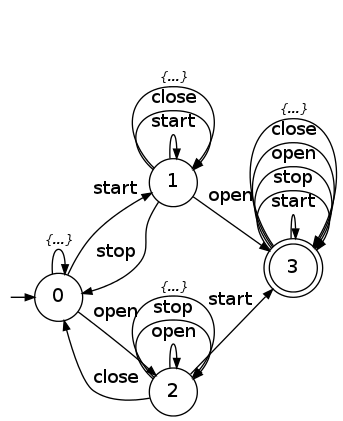
\includegraphics{src/2-framework/images/tester-automaton}}
\scalebox{0.40}{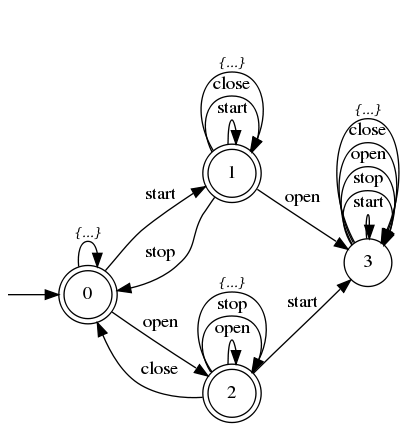
\includegraphics{src/2-framework/images/property-automaton}}
\caption{Tester ($\mathcal{L}^{-}$ at left) and property ($\mathcal{L}^{+}$ at right) automata for \artifact{Maintain[DoorsClosed While Moving]}, as complements of each other.\label{image:tester-and-property-automata}}
\end{figure}

A procedure for computing the tester automaton in the case of safety properties is given in \cite{Giannakopoulou:2003}. Roughly, it consists in composing a B\"uchi automaton that captures the negation of the state-based FLTL property with fluent automata capturing the event-based semantics of fluents, plus a synchronizer between both. 

Given a pure safety property, a canonical form for this automaton can been found; the latter is deterministic, has a complete transition function, and a unique sink accepting state capturing all traces violating the property~\cite{Giannakopoulou:2003}. An example of such tester automaton for the safety goal of the train system is given on the left of Fig.~\ref{image:tester-and-property-automata}. One can check that all traces leading to the accepting state capture situations where the train is moving with doors open. 

The \emph{property} automaton can thus be obtained by flipping accepting and non-accepting states of the tester (as shown on the right of the same figure). 

A few remarks are in order here:

\begin{itemize}

\item In the LTSA tool \cite{Magee:1999} and related literature, a tester LTS with an error state is used instead of the tester automaton presented here. Similarly, \cite{Letier:2005, Letier:2008} actually use a property LTS that corresponds to the tester LTS from which the error state has been removed, instead of the property automaton shown here. Our automata variants are better suited here in view of the formalization of inter-model consistency rules in terms of set-based operators on languages. 

\item The tester and property automata, together with the procedure for computing them, are always defined ``up to a given alphabet'' or ``under the assumption of a given agent or system''. This is the intended meaning of the transitions labeled ``\emph{\{...\}}" in Fig.~\ref{image:tester-and-property-automata}. The reason is that some temporal properties, in particular those referring to the FLTL \emph{next} operator, are not closed under stuttering~\cite{Lamport:1994}. This means that their satisfaction may be affected by the insertion or removal of unobservable events. Which events are relevant depends on additional hypotheses about how goals relate to agent behaviors -- e.g, whether they are under the responsibility of a single agent or are properties to be met by the global system. Fixing those ``relevant events'' by filling the ``\emph{\{...\}}" placeholder is required for meeting the temporal logic semantics when composing tester and property automata. 

For simplicity in the thesis, we will consider that safety properties must be met by the global system. Therefore, the relevant events are the alphabet of the whole system, say $\Sigma$. A placeholder then must be replaced by a transition for each event in $\Sigma$ except those already labeling an outgoing transition on the same state.

\end{itemize}
